%%%%%%%%%%%%%%%%%%%%%%%%%%%%%%%%%%%%%%%%%
% Short Sectioned Assignment
% LaTeX Template
% Version 1.0 (5/5/12)
%
% This template has been downloaded from:
% http://www.LaTeXTemplates.com
%
% Original author:
% Frits Wenneker (http://www.howtotex.com)
%
% License:
% CC BY-NC-SA 3.0 (http://creativecommons.org/licenses/by-nc-sa/3.0/)
%
%%%%%%%%%%%%%%%%%%%%%%%%%%%%%%%%%%%%%%%%%

%----------------------------------------------------------------------------------------
%	PACKAGES AND OTHER DOCUMENT CONFIGURATIONS
%----------------------------------------------------------------------------------------

\documentclass[paper=a4, fontsize=11pt]{scrartcl} % A4 paper and 11pt font size
\usepackage[utf8]{inputenc}
\usepackage[MeX]{polski}
\usepackage[T1]{fontenc} % Use 8-bit encoding that has 256 glyphs
\usepackage{fourier} % Use the Adobe Utopia font for the document - comment this line to return to the LaTeX default
 % English language/hyphenation
\usepackage{amsmath,amsfonts,amsthm} % Math packages
\usepackage{graphicx} %images
\usepackage{placeins}%for direct positioning
\usepackage{lipsum} % Used for inserting dummy 'Lorem ipsum' text into the template

\usepackage{sectsty} % Allows customizing section commands
\allsectionsfont{\centering \normalfont\scshape} % Make all sections centered, the default font and small caps

\usepackage{fancyhdr} % Custom headers and footers
\pagestyle{fancyplain} % Makes all pages in the document conform to the custom headers and footers
\fancyhead{} % No page header - if you want one, create it in the same way as the footers below
\fancyfoot[L]{} % Empty left footer
\fancyfoot[C]{} % Empty center footer
\fancyfoot[R]{\thepage} % Page numbering for right footer
\renewcommand{\headrulewidth}{0pt} % Remove header underlines
\renewcommand{\footrulewidth}{0pt} % Remove footer underlines
\setlength{\headheight}{13.6pt} % Customize the height of the header

\numberwithin{equation}{section} % Number equations within sections (i.e. 1.1, 1.2, 2.1, 2.2 instead of 1, 2, 3, 4)
\numberwithin{figure}{section} % Number figures within sections (i.e. 1.1, 1.2, 2.1, 2.2 instead of 1, 2, 3, 4)
\numberwithin{table}{section} % Number tables within sections (i.e. 1.1, 1.2, 2.1, 2.2 instead of 1, 2, 3, 4)

\setlength\parindent{0pt} % Removes all indentation from paragraphs - comment this line for an assignment with lots of text

%----------------------------------------------------------------------------------------
%	TITLE SECTION
%----------------------------------------------------------------------------------------

\newcommand{\horrule}[1]{\rule{\linewidth}{#1}} % Create horizontal rule command with 1 argument of height

\title{	
\normalfont \normalsize 
\textsc{Uniwersytet Wrocławski} \\ [25pt] % Your university, school and/or department name(s)
\horrule{0.5pt} \\[0.4cm] % Thin top horizontal rule
\huge Naturalna Funkcja Sklejana - Pierwiastki \\
\large Pracownia 2.11 \\ % The assignment title
\horrule{2pt} \\[0.5cm] % Thick bottom horizontal rule
}

\author{Antoni Tomaszewski} % Your name

\date{\normalsize\today} % Today's date or a custom date

\begin{document}

\maketitle % Print the title

%----------------------------------------------------------------------------------------
%	PROBLEM 1
%----------------------------------------------------------------------------------------

\section{Opis problemu}

Tematem zadania jest konstrukcja algorytmu będącego w stanie wyznaczyć pierwiastki równiania $f(x) = c$. Dla zadanych $n+1$ współrzędnych należy zbudować naturalną funkcję sklejaną trzeciego stopnia. Zadanie polega de facto na obliczeniu wartości funkcji odwrotnej $f^{-1}(y)$ w punkcie $y=c$. Niestety funkcja f wcale nie musi być różnowartościowa (ani jakakolwiek z funkcji cząstkowych $s_{k}(x)$). Dlatego do tego problemu zabierzemy się poprzez konstrukcję funkcji sklejanej $s_{k}(x)$ i dla każdego przedziału $[x_{k},x_{k+1}]$ obliczymy pierwiastki równania $s_{k}(x)-c = 0$ % Tutaj nie chcę sk tylko to z indeksem dolnym
\medbreak
Implementacja algorytmu została wykonana w języku Julia w pliku "program.jl".
Funkcje pomocnicze zawarte są w pliku "funkcje.jl''.
Wykresy zostały wygenerowane korzystając z biblioteki "Plots".
Do wygodnego używania wielomianów użyta została biblioteka "Polynomials''.

\section{Naturalnej Funkcji Sklejanej 3 st. - Wyprowadzenie Wzorów}

Mając $n+1$ punktów $(x_{1},y_{1}), (x_{2},y_{2}) ... (x_{n+1}, y_{n+1})$ chcemy na każdym z przedziałów $[x_{k}, x_{k+1}]$ skonstruować wielomian $3$ st. \\
Niech
\begin{gather}
 s_{k}(x) = A_{k} + B_{k}(x - x_{k}) + C_{k}(x - x_{k})^{2} + D_{k}(x - x_{k})^{3} \\
 s_{k}'(x) = B_{k} + 2C_{k}(x - x_{k}) + 3D_{k}(x - x_{k})^{2} \\
 s_{k}''(x) = 2C_{k}+ 6D_{k}(x - x_{k}) \\
 h_{k} = x_{k+1} - x_{k}
\end{gather}
Chcemy więc mieć $n$ funkcji i dla każdej z nich $4$ warunki, co daje w sumie $4n$ warunków. \\
$n+1$ punktów daje nam $2n$ warunków ($n-1$ podwójnych oraz dwa pojedyncze (brzegowe))
Żądamy również, aby pierwsze oraz drugie pochodne na krańcach przedziałów były sobie równe (kolejne $2(n-1)$ warunków).
\begin{align}
s_{k+1}'(x_{k+1}) = s_{k}'(x_{k+1}) \\
s_{k+1}''(x_{k+1}) = s_{k}''(x_{k+1})
\end{align}
Brakuje nam jeszcze dwóch warunków, które zapewniamy sobie ustawiając wartości drugich pochodnych w punktach brzegowych na $0$.
\begin{align}
s_{1}''(x_{1}) = s_{n}''(x_{n+1}) = 0
\end{align}
\\
Skoro $s_{k}(x_{k}) = y_{k}$ mamy więc 
\begin{align}
A_{k} = y_{k}
\end{align}
Korzystając z $(2.7)$ otrzymujemy
\begin{align}
C_{1} = 0 \\
C_{n} + 3D_{n}h_{n} = 0
\end{align}
Licząc 2 pochodną $s_{k+1}''(x_{k+1})$ oraz $s_{k}''(x_{k+1})$ mamy $2C_{k+1} = 2C_{k} + 6D_{k}h_{k}$.
Co daje nam
\begin{align}
D_{k} = \frac{1}{3h_{k}}(C_{k+1} - C_{k})
\end{align}
przy czym $C_{n+1} = 0$ 
\medbreak
Licząc 1 pochodną $s_{k+1}'(x_{k+1}) = B_{k+1}$ oraz $s_{k}'(x_{k+1}) = B_{k} + 2C_{k}h_{k} + 3D_{k}h_{k}^{2}$ \medbreak
Z warunku $(2.5)$ oraz $(2.9)$ mamy
\begin{align}
B_{k+1} = B_{k} +  h_{k}(C_{k+1} + C_{k})
\end{align}
\medbreak
Licząc wartości $s_{k+1}(x_{k+1}) = A_{k+1}$ oraz  $s_{k}(x_{k+1}) = A_{k} + B_{k}h_{k} + C_{k}h_{k}^{2} + D_{k}h_{k}^3$ \medbreak
Co daje wraz z $(2.8)$
\begin{align}
y_{k+1} =  y_{k} + B_{k}h_{k} + C_{k}h_{k}^{2} + D_{k}h_{k}^3
\end{align}
\medbreak
Po skorzystaniu z $(2.11)$ i $(2.9)$ i rozwiązaniu ze względu na $B_{k}$ otrzymujemy:
\begin{align}
B_{k} = \frac{1}{h_{k}}(y_{k+1} - y_{k}) - \frac{h_{k}}{3}(C_{k+1} + 2C_{k})
\end{align}
\medbreak
Korzystając z $(2.12)$ rozpisujemy $B_{k+1}$ i dla wstawiamy obliczone $B_{k+1}$ oraz $B_{k}$ do $(2.10)$
\begin{align*}
B_{k+1} = \frac{1}{h_{k+1}}(y_{k+2} - y_{k+1}) - \frac{h_{k+1}}{3}(C_{k+2} + 2C_{k+1}) \\\\
\frac{y_{k+2} - y_{k+1}}{h_{k+1}} - \frac{y_{k+1} - y_{k}}{h_{k}} = \frac{h_{k+1}}{3}C_{k+2} + \frac{2(h_{k+1} +h_{k})}{3}C_{k+1} + \frac{h_{k}}{3}C_{k} \\\\
h_{k+1} + h_{k} = (x_{k+2} - x_{k+1}) + (x_{k+1} - x_{k}) = x_{k+2} -x_{k} \\
\end{align*}
Po podzieleniu przez $h_{k+1} + h_{k}$ i oznaczeniu $f(x,y,z) = \frac{f(y,z) - f(x,y)}{z-x}$ oraz $f(x,y) = \frac{f(y) - f(x)}{y-x}$ \\
Otrzymujemy dla k $\in$ $1, 2, ..., n-1$
\begin{align}
3f(x_{k}, x_{k+1}, x_{k+2}) = \frac{h_{k+1}}{h_{k+1} + h_{k}}C_{k+2} + 2C_{k+1} + \frac{h_{k}}{h_{k+1} + h_{k}}C_{k}
\end{align}



\section{Pierwiastki $f(x) = c$}

Aby znaleźć wszystkie rozwiązania tego równania możemy przeprować dla każdego z przedziałów $[x_{k}, x_{k+1}]$, poszukiwanie pierwiastków $s_{k}(x) - c = 0$.
A ten problem nie jest trudny. Dzięki wzorom Cardana możemy to zrobić w łatwy sposób.\medbreak
Rówanie $a + bx + cx^2 +dx^3 = 0$ możemy sprowadzić do równania $q + py + y^3 = 0$ (o współczynnikach zespolonych). \medbreak
Przy czym \medbreak
\begin{align}
\begin{cases}
p = \frac{b}{d} - \frac{c^2}{3a^2} \\
q = \frac{2c^3}{27d^3} + \frac{a}{d} - \frac{bc}{3d^2} \\
y = x + \frac{c}{3d}
\end{cases}
\end{align}

Należy jescze rozwiązać układ równań
\begin{align}
\begin{cases}
p = -3uv \\
q = -u^3 - v^3 \\
\end{cases}
\end{align}
Rozwiązania naszego bazowego równania znaleźć teraz możemy aplikując obliczone wartości do wzorów: \medbreak
\begin{align}
\begin{cases}
x_{0} = u + v -\frac{c}{3d} \\
x_{1} = \frac{-u(1+i\sqrt{3})}{2} - \frac{v(1 -i\sqrt{3})}{2} - \frac{d}{3d} \\
x_{2} = \frac{-u(1-i\sqrt{3})}{2} - \frac{v(1 + i\sqrt{3})}{2} - \frac{c}{3d} \\
\end{cases}
\end{align}

Ostatnim etapem w tym rozwiązaniu jest sprawdzenie, które z tych rozwiązań $(x_{0}, x_{1}, x_{2})$ mają część urojoną równą $0$.
Tak obliczone wartości uznajemy za przybliżone wartości spełniające równanie $f(x) = c$.
\begin{figure}[h!]
 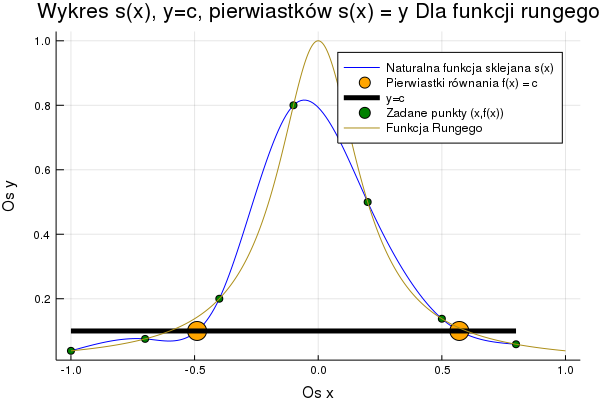
\includegraphics[width=0.95\linewidth]{funkcjarungego.png}
  \caption{Wykres pierwiastków dla funkcji Rungego}
  \label{runge}
\end{figure}
\FloatBarrier


\section{Liczba rozwiązań $f(x) = c$}
Rozważmy inny problem. Niech zadaniem nie będzie znalezienie wszytkich pierwiastków tak zadanego równania, a jedynie wyznaczenie ich ilości. \medbreak
Zauważmy, że na tak sformułowane pytanie jesteśmy w stanie bez trudu odpowiedzieć o ile funkcja jest ciągła i różnowartościowa. \medbreak  \medbreak
Weźmy przedział $[x_{a}, x_{b}]$. \medbreak
Teraz skoro funkcja jest różnowartościowa, wiemy że wartości $f(x_{a}), f(x_{b})$ stanowią minimum oraz maksimum na przedziale. \medbreak 
Bez straty ogólności ustalmy $min = f(x_{a})$ oraz  $max = f(x_{b})$.
 Z ciągłości funkcji $f$ wiemy, że musi ona zawierać wszystkie wartości na przedziale $[min, max]$, a z jej różnowartościowości to że każda z tych wartości występuje dokładnie raz. 
Skoro to już wiemy, jedyne co nam pozostaje to sprawdzić czy $min$ $\leqslant$ $c$ $\leqslant$ $max$. Jeśli tak, na przedziale $[x_{a}, x_{b}]$ istnieje dokładnie jedno rozwiązanie równania $f(x) = c$, w przeciwnym przypadku nie ma go wcale. \medbreak \medbreak

Nasza funkcja $s(x)$ jest ciągła, ale różnowartościwości nie mamy zapewnionej. Wiemy jednak, że na każdym z przedziałów $[x_{k}, x_{k+1}]$ funkcja $s$ równa jest pewnemu wielomianowi 3 st. $s_{k}(x)$. Zauważmy teraz że każdy wielomian 3 st. możemy zawsze podzielić na 3 przedziały, takie że na każdym z nich będzie on różnowartościowy. \medbreak
Weźmy dowolny wielomian $g$ stopnia 3 określony dla wszystkich liczb rzeczywistych, ze współczynnikiem przy najwyższej potędze większym od $0$. \medbreak
Przedziały o które nam chodzi to: \medbreak
 $[-\infty,x_{max}]$, $[x_{max}, x_{min}]$, $[x_{min}, \infty]$, \medbreak
gdzie $x_{max}$ i $x_{min}$ to punkty w których g przyjmuje odpowiednio lokalne maximum oraz minimum \medbreak
Wartości $x_{max}$ i $x_{min}$ możemy uzyskać licząc pierwiastki pochodnej $g'$, która jest wielomianem stopnia 2. \medbreak
(dla współczynniku przy najwyższej potędze $<$ 0 $max$ zamieniamy z $min$, reszta analogiczna)
\medbreak \medbreak
Mając funkcję $s_{k}$ oraz jej $x_{max}$, $x_{min}$ wystarczy więc sprawdzić czy $x_{max}$, $x_{min}$  $\in$ $[x_{k}, x_{k+1}]$. Odpowiednio podzielić ją na 1, 2 lub 3 przedziały i dla każdego z nich przeprowadzić rozumowanie czy $c$ $\in$ $[s_{k}(x_{a}), s_{k}(x_{b})]$. 
Czyli de facto sprawdzić czy $(s_{k}(x_{a}) - c) * (s_{k}(x_{b} - c))$ $\leqslant$ $0$ \medbreak
Przeprowadzając ten algorytm dla $k$ $\in$ $1, 2, ... , n$ otrzymujemy liczbę rozwiązań $s(x) = c$ na przedziale $[x_{1}, x_{n+1}]$. \medbreak \medbreak

Zauważmy że mimo tego, iż algorytm ten nie daje nam odpowiedzi dla jakich $x$, $f(x)=c$, a jedynie ich liczbę, to nie przeszkadza nam w żaden sposób, w razie potrzeby szybko je policzyć ze wzorów wyżej opisanych. Ma on jednak tę wielką zaletę, że jeśli chodzi nam o szybkie wyznaczanie ilości rozwiązań jest on znacznie lepszy, ponieważ pochodne wraz z ich miejscami zerowymi wystarczy policzyć raz i na zapytanie możemy odpowiadać znacznie szybciej. Wystarczy mianowicie dla każdego z maksymalnie $3n$ przedziałów sprawdzić do ilu z nich $c$ należy. Rozwiązanie to daje nam również odpowiedź które to przedziały.
\medbreak
\medbreak
\medbreak
Uwaga!: Algorytm ten liczy pierwiastki podwójne 2 razy, aby uniknąć powtórzeń wystarczy sprawdzać osobno czy zachodzi równość dla lewego punktu brzegowego, dla $x_{n+1}$ oraz nierówność ostra dla punktów wewnątrz przedziału.


\begin{figure}[h!]
 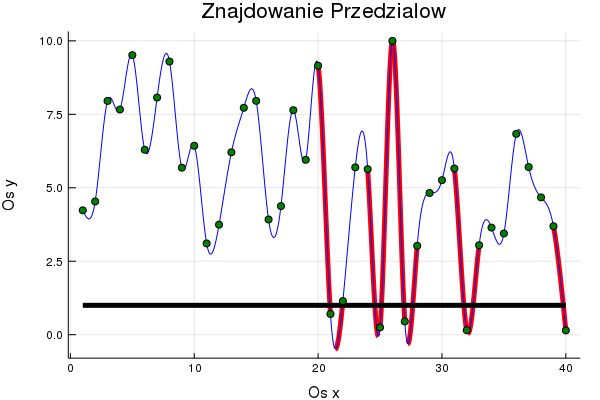
\includegraphics[width=0.95\linewidth]{przedzialy.png}
  \caption{Przedzialy na których $f(x) = c$}
  \label{przedzialy}
\end{figure}
\FloatBarrier


\section{Wnioski}
Przedstawione zostały dwa algorytmy: pierwszy bezpośrednio znajdujący miejsca zerowe funkcji $f(x) - c$, drugi - wyznaczający przedziały na których $f(x) = c$ o długości nie większej niż zadane. Odpowiadają one na inne pytania, a więc wybór metody będzie zależeć od potrzeb. Dla testowanych przykładów, dla żadnego z algorytmów, ani czas, ani pamięć nie stanowiły problemów, ponieważ konstrukcja funkcji sklejanej działa w czasie $O(n)$, a znajdowanie pierwiastków w jednym przedziale w czasie stałym, co daje również złożoność $O(n)$. 

\begin{thebibliography}{9}

\bibitem{splajn}
  Ake Bjorck,
  Germund Dahlquist,
  \textit{Metody Numeryczne}, \\
  Państwowe Wydawnictwo Naukowe, p. 277-280,
  Warszawa 1983

\bibitem{natural}
  David Kincaid,
  Ward Cheney,
  \textit{Analiza Numeryczna}, \\
  Wydawnictwo Naukowo-Techniczne, 
  Warszawa 2006
\end{thebibliography}

\end{document}
